% Options for packages loaded elsewhere
% Options for packages loaded elsewhere
\PassOptionsToPackage{unicode}{hyperref}
\PassOptionsToPackage{hyphens}{url}
\PassOptionsToPackage{dvipsnames,svgnames,x11names}{xcolor}
%
\documentclass[
  11pt,
  letterpaper,
]{article}
\usepackage{xcolor}
\usepackage[margin=1in]{geometry}
\usepackage{amsmath,amssymb}
\setcounter{secnumdepth}{5}
\usepackage{iftex}
\ifPDFTeX
  \usepackage[T1]{fontenc}
  \usepackage[utf8]{inputenc}
  \usepackage{textcomp} % provide euro and other symbols
\else % if luatex or xetex
  \usepackage{unicode-math} % this also loads fontspec
  \defaultfontfeatures{Scale=MatchLowercase}
  \defaultfontfeatures[\rmfamily]{Ligatures=TeX,Scale=1}
\fi
\usepackage{lmodern}
\ifPDFTeX\else
  % xetex/luatex font selection
\fi
% Use upquote if available, for straight quotes in verbatim environments
\IfFileExists{upquote.sty}{\usepackage{upquote}}{}
\IfFileExists{microtype.sty}{% use microtype if available
  \usepackage[]{microtype}
  \UseMicrotypeSet[protrusion]{basicmath} % disable protrusion for tt fonts
}{}
\makeatletter
\@ifundefined{KOMAClassName}{% if non-KOMA class
  \IfFileExists{parskip.sty}{%
    \usepackage{parskip}
  }{% else
    \setlength{\parindent}{0pt}
    \setlength{\parskip}{6pt plus 2pt minus 1pt}}
}{% if KOMA class
  \KOMAoptions{parskip=half}}
\makeatother
% Make \paragraph and \subparagraph free-standing
\makeatletter
\ifx\paragraph\undefined\else
  \let\oldparagraph\paragraph
  \renewcommand{\paragraph}{
    \@ifstar
      \xxxParagraphStar
      \xxxParagraphNoStar
  }
  \newcommand{\xxxParagraphStar}[1]{\oldparagraph*{#1}\mbox{}}
  \newcommand{\xxxParagraphNoStar}[1]{\oldparagraph{#1}\mbox{}}
\fi
\ifx\subparagraph\undefined\else
  \let\oldsubparagraph\subparagraph
  \renewcommand{\subparagraph}{
    \@ifstar
      \xxxSubParagraphStar
      \xxxSubParagraphNoStar
  }
  \newcommand{\xxxSubParagraphStar}[1]{\oldsubparagraph*{#1}\mbox{}}
  \newcommand{\xxxSubParagraphNoStar}[1]{\oldsubparagraph{#1}\mbox{}}
\fi
\makeatother


\usepackage{longtable,booktabs,array}
\newcounter{none} % for unnumbered tables
\usepackage{calc} % for calculating minipage widths
% Correct order of tables after \paragraph or \subparagraph
\usepackage{etoolbox}
\makeatletter
\patchcmd\longtable{\par}{\if@noskipsec\mbox{}\fi\par}{}{}
\makeatother
% Allow footnotes in longtable head/foot
\IfFileExists{footnotehyper.sty}{\usepackage{footnotehyper}}{\usepackage{footnote}}
\makesavenoteenv{longtable}
\usepackage{graphicx}
\makeatletter
\newsavebox\pandoc@box
\newcommand*\pandocbounded[1]{% scales image to fit in text height/width
  \sbox\pandoc@box{#1}%
  \Gscale@div\@tempa{\textheight}{\dimexpr\ht\pandoc@box+\dp\pandoc@box\relax}%
  \Gscale@div\@tempb{\linewidth}{\wd\pandoc@box}%
  \ifdim\@tempb\p@<\@tempa\p@\let\@tempa\@tempb\fi% select the smaller of both
  \ifdim\@tempa\p@<\p@\scalebox{\@tempa}{\usebox\pandoc@box}%
  \else\usebox{\pandoc@box}%
  \fi%
}
% Set default figure placement to htbp
\def\fps@figure{htbp}
\makeatother


% definitions for citeproc citations
\NewDocumentCommand\citeproctext{}{}
\NewDocumentCommand\citeproc{mm}{%
  \begingroup\def\citeproctext{#2}\cite{#1}\endgroup}
\makeatletter
 % allow citations to break across lines
 \let\@cite@ofmt\@firstofone
 % avoid brackets around text for \cite:
 \def\@biblabel#1{}
 \def\@cite#1#2{{#1\if@tempswa , #2\fi}}
\makeatother
\newlength{\cslhangindent}
\setlength{\cslhangindent}{1.5em}
\newlength{\csllabelwidth}
\setlength{\csllabelwidth}{3em}
\newenvironment{CSLReferences}[2] % #1 hanging-indent, #2 entry-spacing
 {\begin{list}{}{%
  \setlength{\itemindent}{0pt}
  \setlength{\leftmargin}{0pt}
  \setlength{\parsep}{0pt}
  % turn on hanging indent if param 1 is 1
  \ifodd #1
   \setlength{\leftmargin}{\cslhangindent}
   \setlength{\itemindent}{-1\cslhangindent}
  \fi
  % set entry spacing
  \setlength{\itemsep}{#2\baselineskip}}}
 {\end{list}}
\usepackage{calc}
\newcommand{\CSLBlock}[1]{\hfill\break\parbox[t]{\linewidth}{\strut\ignorespaces#1\strut}}
\newcommand{\CSLLeftMargin}[1]{\parbox[t]{\csllabelwidth}{\strut#1\strut}}
\newcommand{\CSLRightInline}[1]{\parbox[t]{\linewidth - \csllabelwidth}{\strut#1\strut}}
\newcommand{\CSLIndent}[1]{\hspace{\cslhangindent}#1}



\setlength{\emergencystretch}{3em} % prevent overfull lines

\providecommand{\tightlist}{%
  \setlength{\itemsep}{0pt}\setlength{\parskip}{0pt}}



 


% Wrap the shared author metadata within the printed page width.
\makeatletter
\AtBeginDocument{%
  \let\pocketsolverauthors\@author
  \author{\parbox{0.95\textwidth}{\centering\pocketsolverauthors}}%
}
\makeatother
\makeatletter
\@ifpackageloaded{caption}{}{\usepackage{caption}}
\AtBeginDocument{%
\ifdefined\contentsname
  \renewcommand*\contentsname{Table of contents}
\else
  \newcommand\contentsname{Table of contents}
\fi
\ifdefined\listfigurename
  \renewcommand*\listfigurename{List of Figures}
\else
  \newcommand\listfigurename{List of Figures}
\fi
\ifdefined\listtablename
  \renewcommand*\listtablename{List of Tables}
\else
  \newcommand\listtablename{List of Tables}
\fi
\ifdefined\figurename
  \renewcommand*\figurename{Figure}
\else
  \newcommand\figurename{Figure}
\fi
\ifdefined\tablename
  \renewcommand*\tablename{Table}
\else
  \newcommand\tablename{Table}
\fi
}
\@ifpackageloaded{float}{}{\usepackage{float}}
\floatstyle{ruled}
\@ifundefined{c@chapter}{\newfloat{codelisting}{h}{lop}}{\newfloat{codelisting}{h}{lop}[chapter]}
\floatname{codelisting}{Listing}
\newcommand*\listoflistings{\listof{codelisting}{List of Listings}}
\makeatother
\makeatletter
\makeatother
\makeatletter
\@ifpackageloaded{caption}{}{\usepackage{caption}}
\@ifpackageloaded{subcaption}{}{\usepackage{subcaption}}
\makeatother
\usepackage{bookmark}
\IfFileExists{xurl.sty}{\usepackage{xurl}}{} % add URL line breaks if available
\urlstyle{same}
% fallback for those not using the hyperref driver hyperxmp:
\makeatletter
\@ifundefined{xmpquote}{\newcommand{\xmpquote}[1]{#1}}{}
\makeatother
\hypersetup{
  pdftitle={PocketSolver},
  pdfauthor={Ryan Zheng, Amy Sun, Rain Piao, Connier Wu, Aaron Lee, Nicholas Park, Maksim Fu, Sam Jiang, Emily Du, Justin Zhang, Alexander An, Sumedh Kamat, Jerry Huang},
  colorlinks=true,
  linkcolor={blue},
  filecolor={Maroon},
  citecolor={Blue},
  urlcolor={Blue},
  pdfcreator={LaTeX via pandoc}}


\title{PocketSolver}
\usepackage{etoolbox}
\makeatletter
\providecommand{\subtitle}[1]{% add subtitle to \maketitle
  \apptocmd{\@title}{\par {\large #1 \par}}{}{}
}
\makeatother
\subtitle{Learning to score poker decisions}
\author{{Ryan Zheng}, {Amy Sun}, {Rain Piao}, {Connier Wu}, {Aaron Lee},
{Nicholas Park}, {Maksim Fu}, {Sam Jiang}, {Emily Du}, {Justin Zhang},
{Alexander An}, {Sumedh Kamat}, {Jerry Huang}}
\date{November 13, 2026}
\begin{document}
\maketitle
\begin{abstract}
Poker decisions combine visible cards, betting history, hidden
information, and a changing menu of possible actions. We study a compact
alternative to generating an answer: jointly encode the situation and
its candidate actions, then score each action with a shared prediction
head. We compare four pretrained encoders and two heads on a
10,000-example PokerBench development pool using five scenario-grouped
folds. ModernBERT with a linear head has the highest observed
exact-action agreement, while all eight transformer variants improve log
loss over a linear candidate baseline. We also investigate causal
opponent-history summaries in controlled Leduc forecasting and
observed-action prediction from real Hold'em histories. History improves
the controlled forecasting task, but the current summaries do not
establish a benefit for the Hold'em transformer. PocketSolver makes the
decision model available in an interactive demonstration. These
experiments measure reference or observed action agreement; they do not
establish profitable or unexploitable play.
\end{abstract}


\section{Poker as a structured decision
problem}\label{poker-as-a-structured-decision-problem}

A poker hand asks a deceptively compact question: \textbf{What should
Hero do?} The answer depends on the visible cards, position, pot,
previous actions, and the available choices. Calling and folding are
distinct actions; betting 28 big blinds and betting 51 big blinds are
also distinct actions. A model that chooses the right action type can
still miss the reference by choosing a different amount.

Our starting point is to make those choices explicit. Rather than ask a
language model to write an answer and parse it back into an action, we
supply the candidate actions alongside the situation. The model returns
one score for each candidate. This preserves the exact supplied sizes
and supports menus of different lengths.

Figure~\ref{fig-hand} shows a recorded decision and the scores assigned
by the deployed BERT Mini model. The online explorer includes a postflop
success, a preflop success, and an action-type mistake. They were
selected to illustrate behavior, rather than estimate performance. Each
example was held out by this specific checkpoint.

\begin{figure}[H]

\centering{

\pandocbounded{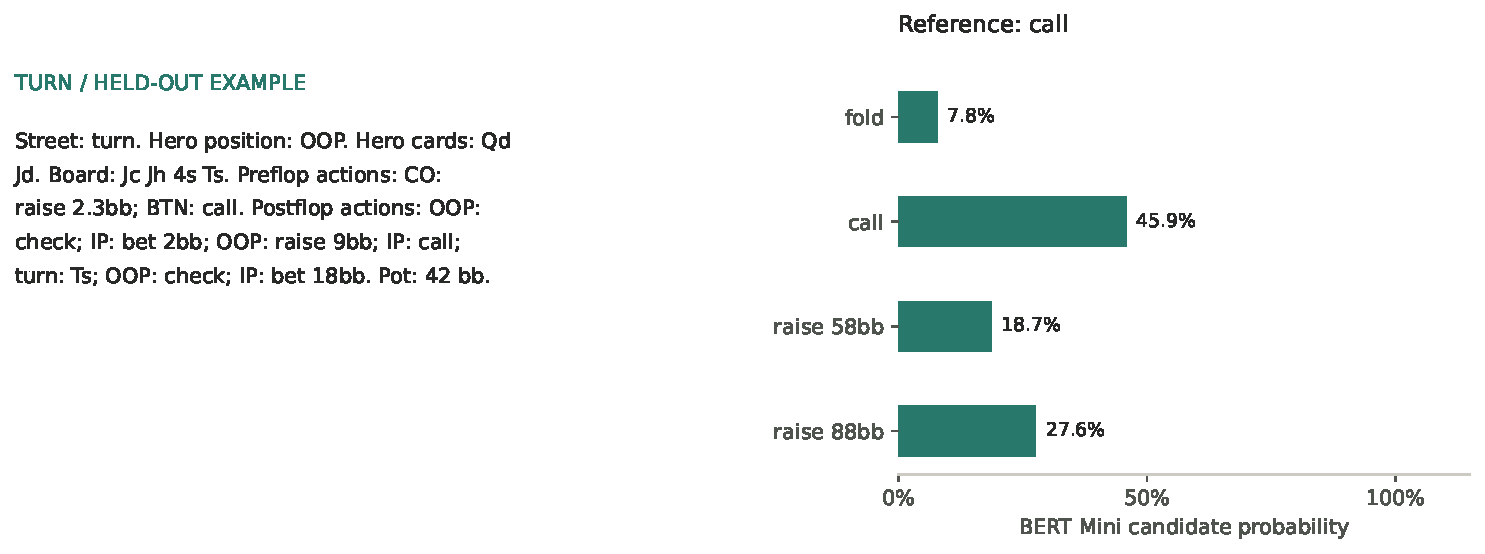
\includegraphics[keepaspectratio]{generated/figures/hand.pdf}}

}

\caption{\label{fig-hand}A held-out decision scored by BERT Mini's
linear head. The printed example matches the explorer's default hand.
Probabilities are a softmax over the supplied actions; they are not
estimated solver mixing frequencies. The online reference is revealed on
request and is excluded from model inputs.}

\end{figure}%

The project separates three questions. First, can a structured encoder
learn to agree with PokerBench reference actions? Second, can previous
behavior help predict an opponent's next action? Third, does appending
those histories improve a transformer on real Hold'em decisions? These
questions use different targets and data, so their scores should be
interpreted within each experiment.

\section{Scoring actions in one forward
pass}\label{scoring-actions-in-one-forward-pass}

\subsection{Joint encoding and a shared
head}\label{joint-encoding-and-a-shared-head}

The input is a context string and an ordered list of candidate actions.
The encoder adapter adds the fixed question, ``What should Hero do?'' We
serialize the state, question, and all candidates into one sequence with
separator tokens. A pretrained encoder produces contextual
representations for every token. For each candidate, we average the
representations of its own tokens and apply the same scoring head.

For candidate \(a_i\) with token positions \(S_i\), the model computes

\[
h_i = \frac{1}{|S_i|}\sum_{t\in S_i} H_t, \qquad
z_i = g_\theta(h_i), \qquad
p(a_i\mid x,A) = \frac{\exp z_i}{\sum_{j\in A}\exp z_j}.
\]

Here \(H\) is the encoder output for the joint sequence and \(A\) is the
supplied menu. The head \(g_\theta\) is either a linear projection or a
two-layer MLP with a ReLU activation. Training updates both the encoder
and head using cross-entropy on the reference candidate index. Candidate
padding is masked before normalization.

\begin{figure}[H]

\centering{

\pandocbounded{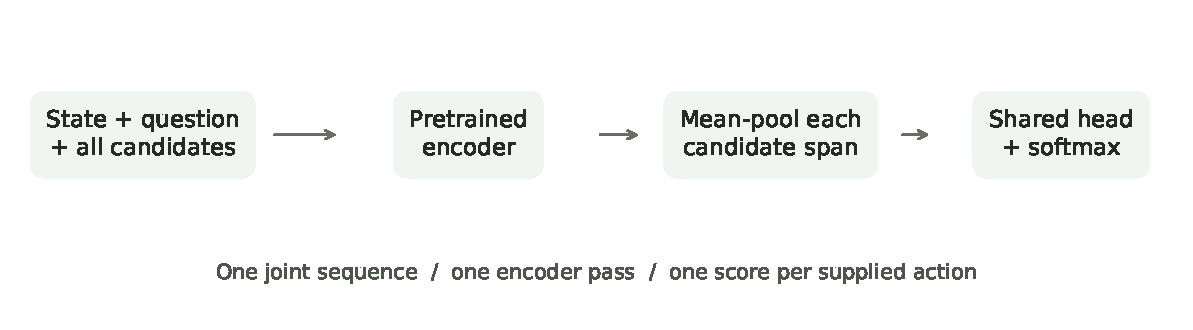
\includegraphics[keepaspectratio]{generated/figures/architecture.pdf}}

}

\caption{\label{fig-architecture}All options share one encoder pass and
one scoring head. Candidate representations can attend to the context
and to other candidates. The web illustration highlights whole action
spans schematically; it does not display exact tokenizer boundaries or
measured attention weights.}

\end{figure}%

The design reuses pretrained language representations in the spirit of
encoder fine-tuning (\citeproc{ref-bert}{Devlin et al. 2019}). It avoids
generating an action token by token, but a single forward pass is not
itself a measured speed advantage. Sequence length, model size,
hardware, batching, and serving overhead all affect latency.

\subsection{What the interface
guarantees}\label{what-the-interface-guarantees}

The input boundary keeps labels and source identifiers separate from
context and candidates. Contexts contain only cards already dealt and
permitted visible information. We do not invent missing stacks or
opponent profiles. Inputs that exceed the configured token limit fail
explicitly rather than silently losing state or candidate tokens.

One limitation follows from joint encoding: candidate order is visible
through positional encodings. Sharing a head does not make the model
permutation invariant. Candidate-order augmentation and explicit
order-robustness evaluation remain natural follow-up experiments. The
model can choose only among the supplied candidates; it does not
establish that those candidates exhaust legal or useful poker actions.

\section{Evaluating beyond repeated
scenarios}\label{evaluating-beyond-repeated-scenarios}

\subsection{Sources and splits}\label{sources-and-splits}

Our primary action-choice experiment uses the pinned PokerBench training
sources (\citeproc{ref-pokerbench}{Zhuang et al. 2025}). The source
audit validates 63,200 preflop rows and 500,000 postflop rows. The
development working pool samples 5,000 examples from each source, giving
10,000 examples in total. This sampling balance describes the
experiment; it is not an estimate of the frequency of these situations
in play.

An early walkthrough used a context-grouped 8,000/2,000 split. Identical
contexts never crossed that boundary, but related scenarios often did:
91.8\% of validation rows had a scenario group represented in training.
We therefore use a broader, answer-free scenario grouping for the model
comparison reported here.

Preflop groups use the full previous betting history. Postflop groups
use the sorted ranks of the first three board cards, keeping suit
variants and later streets together. Across the five maintained folds,
neither specified scenario groups nor exact contexts overlap between
training and held-out examples. Every example receives exactly one
held-out prediction per model. This grouping is a specific stress test;
it cannot establish independence under every possible notion of poker
similarity.

\begin{longtable}[]{@{}
  >{\raggedleft\arraybackslash}p{(\linewidth - 6\tabcolsep) * \real{0.2500}}
  >{\raggedleft\arraybackslash}p{(\linewidth - 6\tabcolsep) * \real{0.2500}}
  >{\raggedleft\arraybackslash}p{(\linewidth - 6\tabcolsep) * \real{0.2500}}
  >{\raggedleft\arraybackslash}p{(\linewidth - 6\tabcolsep) * \real{0.2500}}@{}}
\caption{Five fixed development folds. Groups are defined without
reference labels.}\label{tbl-folds}\tabularnewline
\toprule\noalign{}
\begin{minipage}[b]{\linewidth}\raggedleft
Fold
\end{minipage} & \begin{minipage}[b]{\linewidth}\raggedleft
Training examples
\end{minipage} & \begin{minipage}[b]{\linewidth}\raggedleft
Held-out examples
\end{minipage} & \begin{minipage}[b]{\linewidth}\raggedleft
Shared scenario groups
\end{minipage} \\
\midrule\noalign{}
\endfirsthead
\toprule\noalign{}
\begin{minipage}[b]{\linewidth}\raggedleft
Fold
\end{minipage} & \begin{minipage}[b]{\linewidth}\raggedleft
Training examples
\end{minipage} & \begin{minipage}[b]{\linewidth}\raggedleft
Held-out examples
\end{minipage} & \begin{minipage}[b]{\linewidth}\raggedleft
Shared scenario groups
\end{minipage} \\
\midrule\noalign{}
\endhead
\bottomrule\noalign{}
\endlastfoot
1 & 8,070 & 1,930 & 0 \\
2 & 7,889 & 2,111 & 0 \\
3 & 8,067 & 1,933 & 0 \\
4 & 7,911 & 2,089 & 0 \\
5 & 8,063 & 1,937 & 0 \\
\end{longtable}

\subsection{Baselines, training, and
metrics}\label{baselines-training-and-metrics}

We compare uniform candidate probabilities, a training-only option
prior, and a linear candidate model with four pretrained encoders: BERT
Mini, MiniLM, DistilBERT, and ModernBERT. Each encoder receives both a
linear head and an MLP head, for eight transformer configurations and 40
fitted folds.

Every transformer fit uses seed 42, three fixed epochs, batch size 16,
encoder learning rate \(2\times10^{-5}\), head learning rate
\(10^{-3}\), weight decay 0.01, and maximum sequence length 512. The MLP
width is 64. Each fold starts with a fresh encoder, head, and optimizer.
Held-out folds do not choose epochs. Baselines are refitted using each
fold's training examples.

\textbf{Exact accuracy} measures agreement with the supplied reference
candidate, including its amount. \textbf{Log loss} measures the
probability assigned to that reference and penalizes confident mistakes.
We also record action-type macro-F1, Brier score, street-specific
performance, and multi-option accuracy. The latter excludes decisions
with only one candidate, which require no choice; such rows make up
4.64\% of the pool. Uniform probabilities have ties, so deterministic
exact accuracy and tie-expected accuracy can differ.

These are development comparisons on an inspected pool, with one
training seed. Selecting a model from this matrix and quoting the same
score does not provide an independent final performance estimate. The
maintained workflows do not load the official test, but some original
team submissions had already inspected it. An independent evaluation
needs a predeclared new holdout or nested selection.

\section{What do the models learn?}\label{what-do-the-models-learn}

\subsection{Better probability quality, modest accuracy
gains}\label{better-probability-quality-modest-accuracy-gains}

ModernBERT with a linear head has the highest observed exact accuracy,
71.92\%, and the lowest log loss, 0.6078. The linear candidate baseline
reaches 69.69\% accuracy and 1.0025 log loss. The observed accuracy
improvement is 2.23 percentage points.

\begin{figure}[H]

\centering{

\pandocbounded{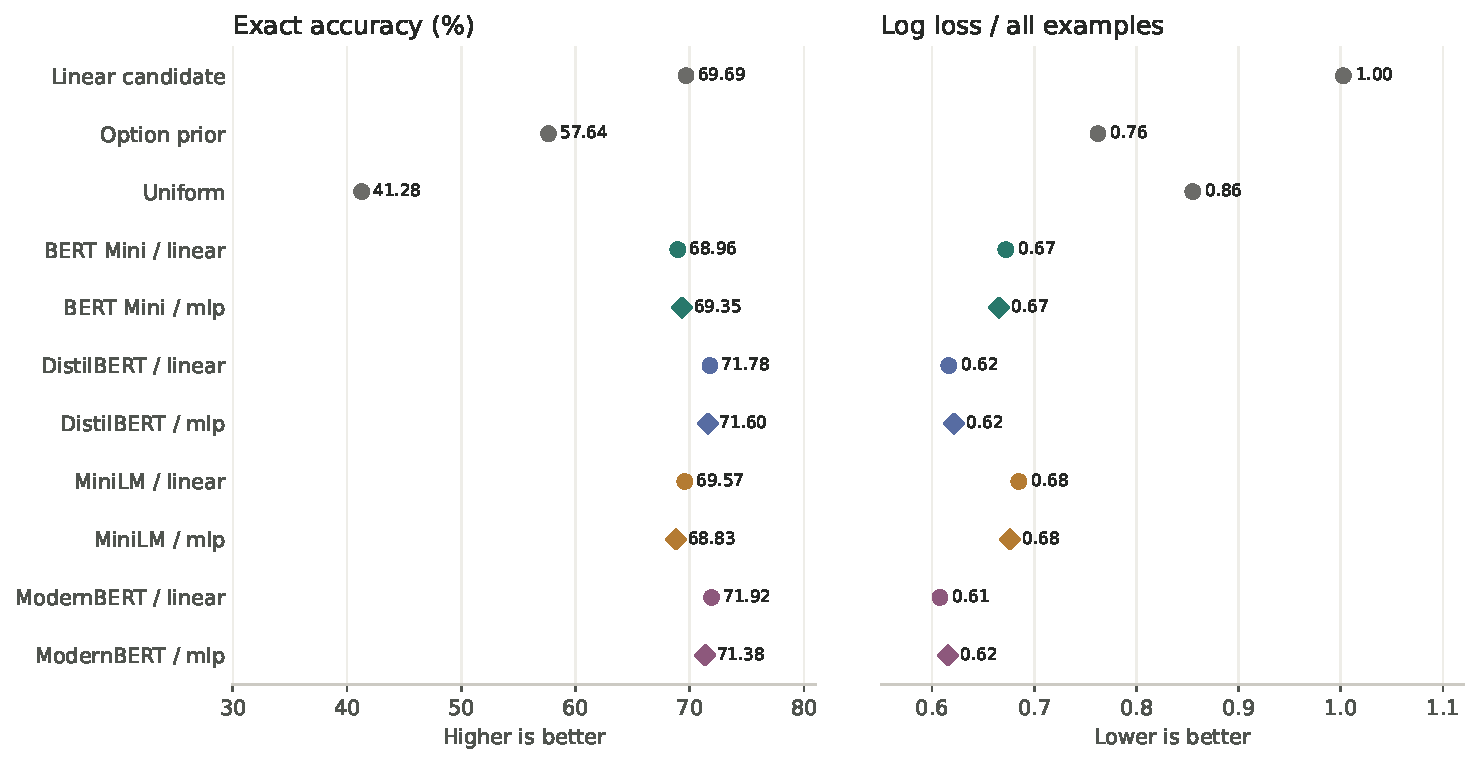
\includegraphics[keepaspectratio]{generated/figures/models.pdf}}

}

\caption{\label{fig-models}Development comparison on 10,000 examples,
with one held-out prediction per model and example. Circles denote
linear heads and diamonds MLP heads for transformers. Higher accuracy
and lower log loss are better. The web control changes only the accuracy
panel to exclude single-option rows; log loss remains over all examples.
No plotted uncertainty bars are implied by these point estimates.}

\end{figure}%

DistilBERT linear reaches 71.78\%, only 14 decisions behind ModernBERT
out of 10,000. That small gap does not establish a reliable advantage
for ModernBERT. Adding an MLP does not consistently improve either
metric across encoders. BERT Mini and MiniLM do not beat the linear
candidate baseline on exact accuracy in these runs, although all eight
transformer configurations have lower log loss.

This distinction matters. A model can make a similar number of
top-choice mistakes while distributing its remaining probability more
usefully. Lower log loss is evidence about reference-label probability
quality. It does not establish that the softmax is calibrated or that it
recovers an optimal mixed strategy.

The saved paired scenario-group bootstrap interval for ModernBERT
linear's accuracy gain over the linear candidate baseline is
approximately +1.01 to +3.33 percentage points. That interval conditions
on the saved fitted models and specified groups; it excludes variation
from retraining and cannot remove the consequences of selecting a model
after inspecting development results.

\subsection{Street-level behavior and illustrative
mistakes}\label{street-level-behavior-and-illustrative-mistakes}

An overall average conceals substantial variation between streets.
Figure~\ref{fig-streets} compares the deployed BERT Mini architecture
and ModernBERT, using linear heads. Preflop agreement is higher than
postflop agreement in these runs. Street counts are uneven: there are
5,000 preflop, 310 flop, 2,021 turn, and 2,669 river decisions. We
should avoid attributing those differences to a single mechanism without
controlled experiments on the representation, menus, and source
distributions.

\begin{figure}[H]

\centering{

\pandocbounded{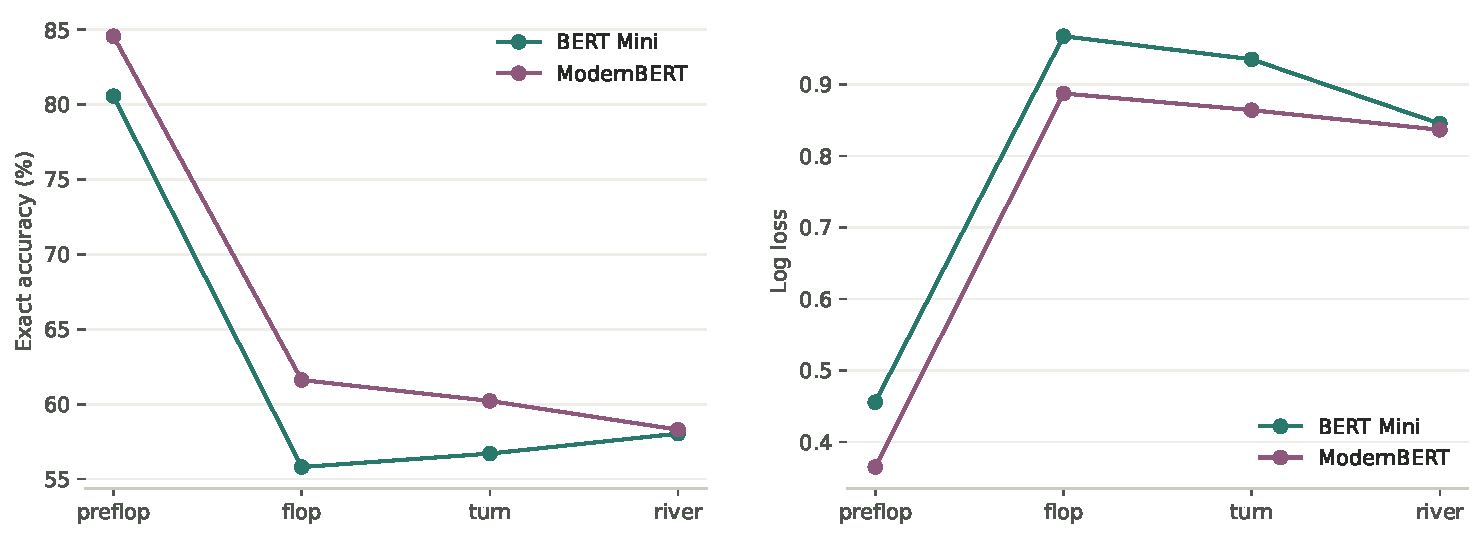
\includegraphics[keepaspectratio]{generated/figures/streets.pdf}}

}

\caption{\label{fig-streets}Street-specific exact accuracy and log loss
from the same held-out development predictions. Connected points
organize categorical streets; they do not describe a learning
trajectory.}

\end{figure}%

The hand explorer in Figure~\ref{fig-hand} complements aggregate metrics
by exposing an actual action-type error. It also permits comparison with
the saved linear baseline on exactly the same input. These examples are
purposefully selected. The available 256-hand demo sample contains no
wrong-amount errors for this checkpoint, so that category is not
illustrated here. The broader evaluation supports separating amount
errors from action-type errors, but a representative error taxonomy
requires the full saved decision pool and its declared selection rules.

\section{Does opponent history help?}\label{does-opponent-history-help}

\subsection{Controlled forecasting in
Leduc}\label{controlled-forecasting-in-leduc}

The first history experiment isolates opponent-action forecasting in a
small, controlled game. We generate Leduc sessions with five policy
profiles: tight, passive, aggressive, balanced, and switching. Fifty
opponent instances play two sessions each, giving 6,000 hands and 12,711
recorded decisions. Repeated sessions from one opponent stay in the same
split.

Predictors receive the observer's own private rank, public board, pot
and contributions, legal menu, and current public action prefix.
Opponent private cards and generator metadata are excluded. History
summaries use completed previous hands and match the relevant action
opportunities. They cannot look at future hands or the current target.

\begin{figure}[H]

\centering{

\pandocbounded{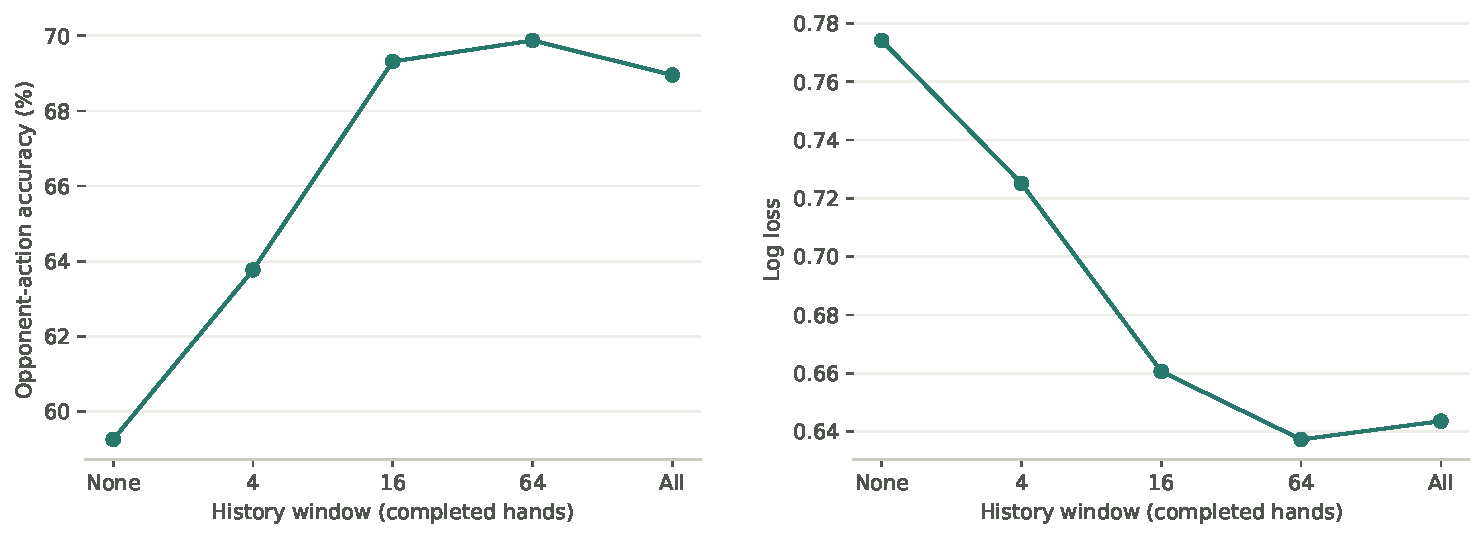
\includegraphics[keepaspectratio]{generated/figures/leduc.pdf}}

}

\caption{\label{fig-leduc}Controlled Leduc opponent-action forecasting
on 2,506 held-out decisions from 10 opponents. History windows are
counts of completed hands. The 64-hand primary window was selected using
validation log loss; the plotted test points are descriptive comparisons
within this one simulated population.}

\end{figure}%

The masked logistic forecaster improves from 59.26\% to 69.87\% accuracy
when given the selected history summary, while log loss falls from
0.7741 to 0.6373. The paired whole-opponent bootstrap accuracy interval
is +3.42 to +18.97 percentage points, conditional on the fitted models
and generated population.

More history is not uniformly better. All-history summaries are slightly
worse than the selected 64-hand window, and history-based models can lag
after a policy switch. The first-five-hands-after-switch slice contains
only 40 decisions from two opponent instances, so it is descriptive.
These results motivate studying memory under behavior changes; they do
not establish human tilt detection or better Hero decisions.

\subsection{Connecting histories to real Hold'em
inputs}\label{connecting-histories-to-real-holdem-inputs}

We next reuse causal summaries with replayed Hold'em histories from the
Pluribus setting (\citeproc{ref-pluribus}{Brown and Sandholm 2019}). The
target here is the observed human action. This differs from PokerBench
reference-action imitation and from the simulated Leduc task. The
transformer receives a summary of completed-hand opponent behavior
appended to its input. Learned forecaster probabilities are not injected
into the model.

The follow-up uses nested training samples of 128, 1,024, and 4,096
decisions and the same 1,024 validation decisions. The
numeric-session-group split, initialization, seed, learning rates, and
one-epoch budget remain fixed. Validation does not select an epoch or
hyperparameter. The public-state forecaster and BERT Mini have different
information boundaries, so their panels are separate matched ablations.

\begin{figure}[H]

\centering{

\pandocbounded{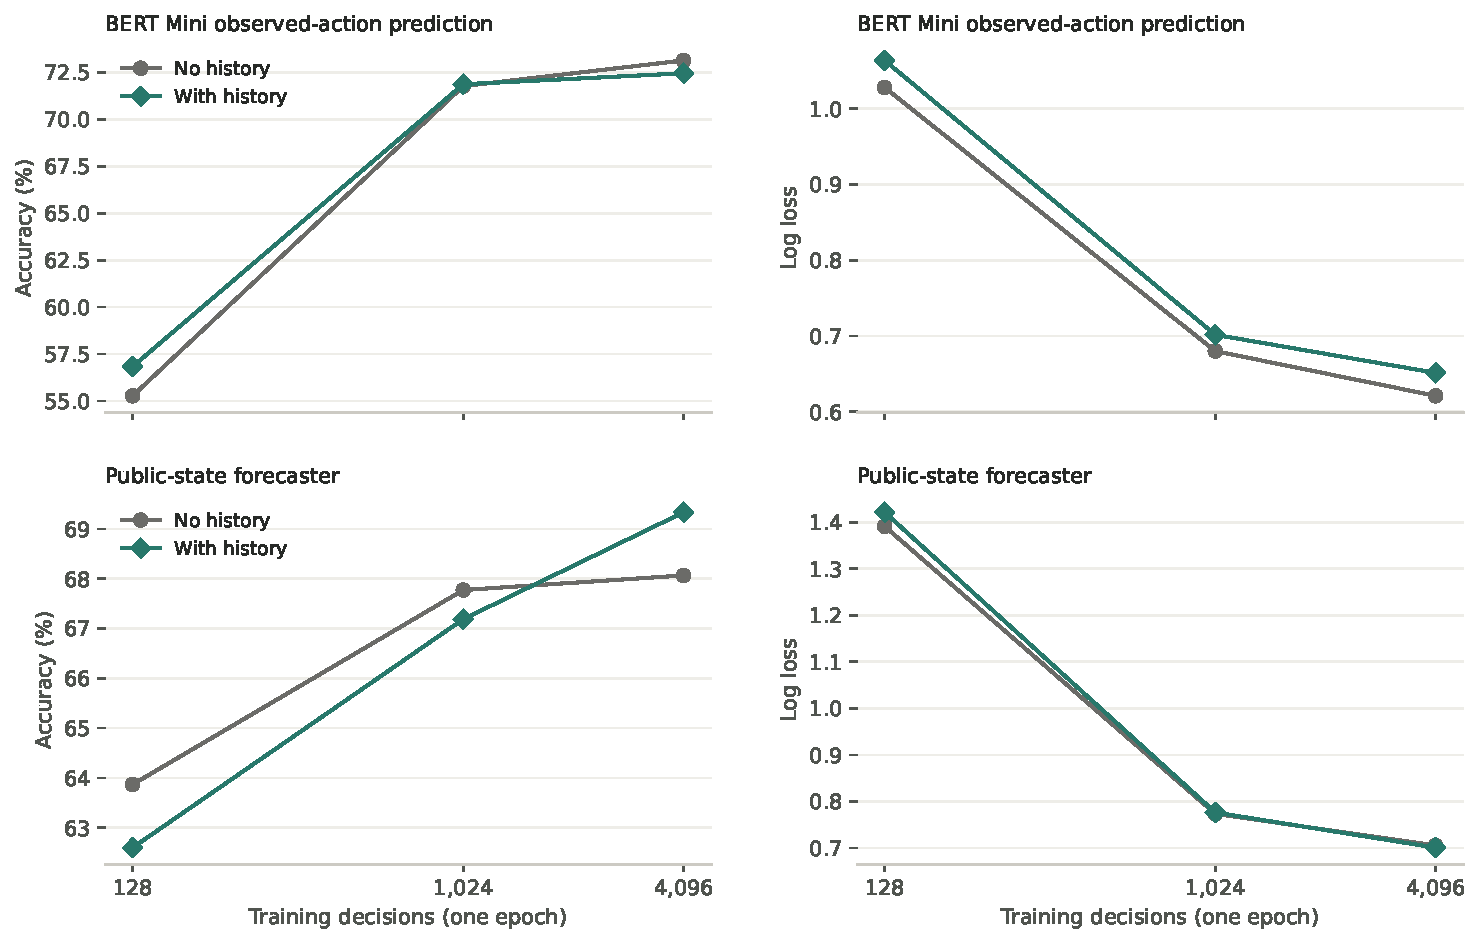
\includegraphics[keepaspectratio]{generated/figures/holdem.pdf}}

}

\caption{\label{fig-holdem}History ablations across nested training
sizes on the same 1,024 Hold'em validation decisions. The top row shows
BERT Mini observed-action prediction; the bottom row shows the
public-state forecaster. Each matched pair varies history availability.
One epoch on a larger sample entails more optimizer steps, so this is
not an equal-compute comparison.}

\end{figure}%

More training substantially improves prediction, but the appended
summaries do not establish a transformer benefit. At 4,096 training
decisions, accuracy is 73.14\% without history and 72.46\% with history.
Log loss rises from 0.621108 to 0.651398. The paired session-cluster
interval for the accuracy change is -2.51 to +1.04 percentage points.
The apparent history gain in the original 64-example integration check
does not persist in the larger comparison.

The public-state forecaster shows a smaller, different result. At 4,096
training decisions, history increases accuracy from 68.07\% to 69.34\%
and reduces log loss from 0.705272 to 0.700675. Its paired log-loss
interval is -0.008054 to -0.001070. This supports a modest conditional
forecasting benefit, while leaving the transformer integration question
open.

These experiments use one seed, an inspected validation set, and
recurring human aliases across different sessions. Session-cluster
intervals do not capture retraining variation or generalization to
unseen players. A useful next experiment would vary summary
representation and memory while preserving paired memberships, then
evaluate a predeclared configuration on new sessions or players.

\section{Explore PocketSolver}\label{explore-pocketsolver}

PocketSolver restores the trained BERT Mini encoder and linear candidate
head on CPU. Its 256-hand sample consists of multi-option decisions held
out by that checkpoint. The reference appears after prediction and is
excluded from both model and live LLM inputs. The small checkpoint is a
serving choice; it is not the highest-scoring model in the development
matrix.

The interactive application is available at
\href{https://www.nmokey.com/poker/}{www.nmokey.com/poker}. The online
article also contains a recorded hand explorer that does not require
live inference.

The live comparison is an illustration, not a controlled
model-versus-LLM study. Provider failures and allowance limits remain
visible. A few hands or one browser timing cannot establish general
quality or latency advantages. A proper serving comparison should record
hardware, cold and warm execution, input lengths, provider settings,
successful-response coverage, and repeated measurements.

\section{Limitations and next steps}\label{limitations-and-next-steps}

The strongest supported conclusion is narrow: jointly encoding a
situation and its candidate actions is a workable supervised interface,
and the larger encoders improve reference-label probability quality with
modest accuracy gains over a strong simple baseline. Causal opponent
summaries help in one controlled forecasting setting, while their
current Hold'em transformer integration does not show a reliable gain.

Several limitations determine what to do next. Independent final
evaluation and multiple training seeds would clarify how much of the
observed ranking persists. Candidate-order perturbations and
representation ablations would test whether models depend on incidental
serialization or menu shortcuts. Calibration should be fitted and
assessed on data separate from final evaluation. Controlled serving
measurements would test the practical benefit of avoiding autoregressive
output.

Finally, agreement with one reference action is not a payoff evaluation.
A single label does not describe a full solver strategy, and observed
human actions need not be optimal. Claims about profitable, robust, or
unexploitable play require additional repeated-play or game-theoretic
evaluation. The present article and demo provide a reproducible
foundation for those experiments.

\section{Reproducibility and complete
results}\label{reproducibility-and-complete-results}

All reported comparisons use saved protocols and reviewed aggregate
results. The report build validates the main CSV against the
corresponding JSON, checks the demo hand checksum, and joins examples to
the saved fold-specific predictions. It exports the same figures as SVG
for the web and vector PDF for LaTeX, together with source and output
hashes. No training or live inference runs while rendering the article.

The manuscript, bibliography, shared values, and figure identifiers are
common to HTML, PDF, and LaTeX. The print hand and model figures match
the default web states. Web-only controls supplement the paper's
argument without carrying claims that are absent from the static
version.

\begin{longtable}[]{@{}llrrr@{}}
\caption{Complete development matrix. Multi-option accuracy excludes
single-candidate rows. Uniform exact accuracy uses the evaluator's
deterministic tie rule; tie-expected accuracy is 44.57\% overall. All
rows cover the same working pool.}\label{tbl-models}\tabularnewline
\toprule\noalign{}
Model & Head & Exact accuracy & Multi-option accuracy & Log loss \\
\midrule\noalign{}
\endfirsthead
\toprule\noalign{}
Model & Head & Exact accuracy & Multi-option accuracy & Log loss \\
\midrule\noalign{}
\endhead
\bottomrule\noalign{}
\endlastfoot
Linear candidate & --- & 69.69\% & 68.22\% & 1.0025 \\
Option prior & --- & 57.64\% & 55.58\% & 0.7623 \\
Uniform & --- & 41.28\% & 38.42\% & 0.8551 \\
BERT Mini & linear & 68.96\% & 67.45\% & 0.6722 \\
BERT Mini & mlp & 69.35\% & 67.86\% & 0.6656 \\
DistilBERT & linear & 71.78\% & 70.41\% & 0.6164 \\
DistilBERT & mlp & 71.60\% & 70.22\% & 0.6213 \\
MiniLM & linear & 69.57\% & 68.09\% & 0.6849 \\
MiniLM & mlp & 68.83\% & 67.31\% & 0.6764 \\
ModernBERT & linear & 71.92\% & 70.55\% & 0.6078 \\
ModernBERT & mlp & 71.38\% & 69.99\% & 0.6158 \\
\end{longtable}

The repository contains the detailed
\href{https://github.com/nmokey/Poker-Decision-Model/blob/main/docs/week2-results.md}{model
protocol},
\href{https://github.com/nmokey/Poker-Decision-Model/blob/main/docs/scientific-audit.md}{scientific
audit},
\href{https://github.com/nmokey/Poker-Decision-Model/blob/main/docs/meeting4-results.md}{Leduc
experiment}, and
\href{https://github.com/nmokey/Poker-Decision-Model/blob/main/docs/meeting5-scaling.md}{Hold'em
follow-up}. The local draft may precede publication of those files on
the repository's default branch. The generated provenance file
identifies the exact local sources used.

\section*{References}\label{references}
\addcontentsline{toc}{section}{References}

\protect\phantomsection\label{refs}
\begin{CSLReferences}{1}{1}
\bibitem[\citeproctext]{ref-pluribus}
Brown, Noam, and Tuomas Sandholm. 2019. {``Superhuman {AI} for
Multiplayer Poker.''} \emph{Science} 365 (6456): 885--90.
\url{https://doi.org/10.1126/science.aay2400}.

\bibitem[\citeproctext]{ref-bert}
Devlin, Jacob, Ming-Wei Chang, Kenton Lee, and Kristina Toutanova. 2019.
\emph{{BERT}: Pre-Training of Deep Bidirectional Transformers for
Language Understanding}. \url{https://arxiv.org/abs/1810.04805}.

\bibitem[\citeproctext]{ref-pokerbench}
Zhuang, Richard, Akshat Gupta, Richard Yang, Aniket Rahane, Zhengyu Li,
and Gopala Anumanchipalli. 2025. \emph{{PokerBench}: Training Large
Language Models to Become Professional Poker Players}.
\url{https://arxiv.org/abs/2501.08328}.

\end{CSLReferences}




\end{document}
